%-------------------------------------------------------------------------------------------------------
%
%
%
%-------------------------------------------------------------------------------------------------------    
\unnumberedChapter{The LCS Node Model}

This chapter introduces the concepts used by firmware to describe and control a layout. Hardware modules provide the physical interface to the layout, while their firmware presents a consistent logical model to the Layout Control System (LCS). The key elements of that model are nodes, ports, channels, attributes, items, and events.

Together, these concepts support two complementary ways of working with a layout. Resources can be addressed directly when a specific node, port, or channel must be configured or controlled. Alternatively, nodes can interact through broadcast events, allowing sensors and actors to be connected in a producer/consumer model.


\unnumberedSection{Nodes}

A \textbf{node} is the logical representation of a hardware module within the layout control system. Each node is uniquely identified by a \textbf{node ID}. A node ID can be assigned automatically by a central component in response to a request, or it can be assigned manually. Node IDs are used whenever a message must address a particular node directly. The number itself has no inherent classification or meaning; if categories or ranges are useful, they are defined by the configuration system.

Every node also has a \textbf{node type}, which describes the functions the node can perform. Examples include a base station, booster, turnout module, or signal-control module. Because the node type reflects the capabilities of the underlying hardware, it normally changes only when the hardware changes. Once a node has been assigned a node ID, configuration tools can use configuration messages to set its variables and operating parameters.

Each node maintains a \textbf{node map}. This map contains the information required to configure the node, including its unique ID, its type, and the number of ports it provides. The map is stored in non-volatile memory so that the node can restore its configuration after a power cycle. A node map can be initialized with default values when a module is new, has previously been used in another layout, or requires a revised map format after a firmware update. The same mechanism is used when assigning a new node ID.

\unnumberedSection{Ports}

A node provides one or more receiving and control endpoints, called \textbf{ports}. A node can support up to eight ports. Ports form the connection between the physical hardware and the software model: an output that drives a turnout, for example, can be represented as a port on a node. When a message or event addresses that port, the node firmware performs the corresponding action.

Each node has a \textbf{port map} with one entry for every port. A \textbf{port-map entry} records the port's configuration, state, and type. It also contains a small set of user-definable attributes that firmware can use for port-specific data, such as a hardware pin assignment, an operating mode, or a limit value.

\unnumberedSection{Channels}

A port may be divided further into \textbf{channels}. Each port can support up to eight channels. A channel is the smallest directly addressable unit in the layout. Individual signal heads, turnouts, and track sections are typical examples.

The combination of node ID, port number, and channel number forms a unique LCS address. With up to 1,023 nodes, eight ports per node, and eight channels per port, the system can address well over 60,000 individual channels.

\unnumberedSection{Addressing}

Direct addressing identifies a specific resource by its node, port, and, where applicable, channel. It is used whenever a configuration tool or another node must read or change a particular resource. For example, a control panel may directly set a turnout connected to a specified node and port.

\begin{center}
      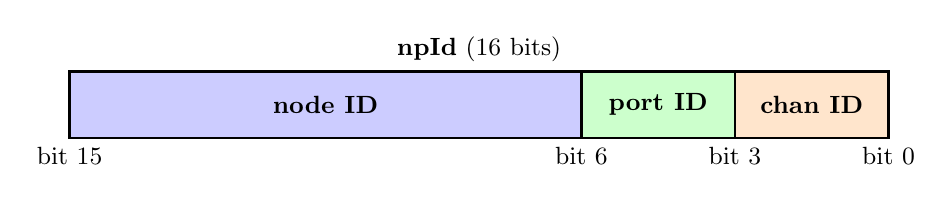
\begin{tikzpicture}[font=\small, x=0.65cm, y=0.7cm]
        % A 16-bit npId: node ID [15:6], port ID [5:3], channel ID [2:0]
        \fill[blue!20] (0,0) rectangle (10,1.2);
        \fill[green!20] (10,0) rectangle (13,1.2);
        \fill[orange!20] (13,0) rectangle (16,1.2);
        \draw[thick] (0,0) rectangle (16,1.2);
        \draw[thick] (10,0) -- (10,1.2);
        \draw[thick] (13,0) -- (13,1.2);

        \node at (5,0.6) {\textbf{node ID}};
        \node at (11.5,0.6) {\textbf{port ID}};
        \node at (14.5,0.6) {\textbf{chan ID}};

        \node[below] at (0,0) {bit 15};
        \node[below] at (10,0) {bit 6};
        \node[below] at (13,0) {bit 3};
        \node[below] at (16,0) {bit 0};
        \node[above] at (8,1.2) {\textbf{npId} (16 bits)};
   \end{tikzpicture}
\end{center}

This direct model of addressing is deliberately separate from event processing. It provides a precise interface for configuration and explicit control, even when the same physical action could also be initiated by an event.

\unnumberedSection{Attributes, Functions and Items}

\textbf{Node attributes}, \textbf{port attributes}, and \textbf{channel attributes} are variables that can be read or set. LCS represents attribute access and function operations through \textbf{items}: numeric identifiers that are accompanied by parameter data when needed. The parameter data qualifies the requested item or carries the value to be written.

The item-number range is divided into a reserved range for functions defined by LCS and a user-defined range. The user-defined range provides flexibility for the specialized functions of a particular node or port; its meaning is determined by the firmware designer. For example, an occupancy-detector module might provide an attribute that reports the current state of its block sections. A block controller might provide an item request that turns track power on or off, with a parameter specifying the desired state.

The LCS Runtime Library handles as much of this processing as possible without involving the upper firmware layer. For example, when another node sends a request to read or write a standard attribute, the runtime validates the request, accesses the appropriate map entry, and sends the response transparently. The module-specific firmware does not need to implement this protocol handling.

User-defined functions follow a different path. When the runtime receives a request for a user-defined function, it passes the request to the upper firmware through a callback. The module firmware then performs the specialized action and, where necessary, supplies a result. This division of responsibility is intentional: the runtime handles common communication and storage mechanics, allowing the module firmware to concentrate on the functions that are specific to the hardware it controls.

\unnumberedSection{Events}

The LCS bus, hardware modules, nodes, ports, and channels describe the statically configured structure of a layout. Attribute access provides direct interaction with a specific node and item. Events provide the complementary producer/consumer model through which nodes can react to one another without being addressed directly.

An \textbf{event} is a message broadcast by a node on the LCS bus. Every node receives the message; nodes that are configured to recognize that event act on it. The transmitting node is the \textbf{producer}, and the responding node is the \textbf{consumer}. Multiple producers may broadcast the same event, and multiple consumers may react to it.

Each event has a unique 16-bit \textbf{event ID}, assigned by a configuration tool. The ID is arbitrary apart from its uniqueness, providing 65,536 possible events. Each node maintains an \textbf{event map}, which contains an entry for every event-ID/port-ID combination to which the node responds. Because the event itself identifies the relationship, a consumer does not need to know the node ID of the producer.

To connect a producer and a consumer, both must be configured with the same event ID. An outbound port is configured to broadcast an event when a particular condition is observed. For example, a front-panel push button can broadcast a selected event ID when it is pressed. An inbound port is configured with the event IDs it recognizes and the action it should take when each is received. An inbound port may listen for many events, whereas an outbound port broadcasts exactly one event ID for a given observation or action.

Direct addressing remains necessary for two reasons. First, configuration messages must reach the particular node and port whose attributes or event-map entries are being changed. Second, direct addressing is useful for explicit control of a resource, such as setting a turnout. The same operation could be modeled as an event, but a dedicated node/port address is often simpler to configure and clearer to use.


\unnumberedSection{Configuration Mode}

Before normal operation begins, nodes, ports, channels, attributes, and events must be configured. Once a node has a valid node ID, configuration consists of sending it the global and port-specific information it needs, including port-map and event-map entries. The node stores this information in non-volatile memory so that it can restore a consistent configuration at the next power-up.

Values may change during operation, but the node retains its configured state as the startup baseline. Configuration primarily assigns item and event IDs to functions, producers, and consumers. The firmware defines a node's capabilities; attributes and events then define its static configuration and dynamic behavior. Installing a new firmware version is an explicit operation and is separate from configuration.


\unnumberedSection{Operation Mode}

The task of a layout control system is to manage the layout's sensors and actors. LCS does this through direct attribute access and event broadcasting. It controls and monitors stationary equipment such as signals, turnouts, detectors, and track sections, while the DCC subsystem is responsible for controlling mobile decoders in locomotives and other rolling stock.

A layout commonly contains one or more track sections, each managed by a booster or block-controller node. These sections can be monitored for power consumption to detect short circuits. Feedback technologies such as RailCom can be handled by the booster node and can provide information about the rolling stock on the track. Occupancy detectors, turnout-position detectors, signals, and other stationary equipment are monitored or controlled through LCS messages and events.

Conceptually, any node can send or receive event, information, or control messages. Base stations, cab handhelds, boosters, and other devices are all LCS nodes with different node types and firmware functions.


\unnumberedSection{Summary}

This chapter introduced the basic concepts of the layout control system. LCS separates the control of mobile equipment from the control of stationary layout elements. Mobile decoders are controlled by the DCC subsystem; communication with the remaining hardware takes place on the LCS bus, to which all hardware modules connect.

Hardware modules host nodes. The current implementation hosts one node per hardware module. A node contains one or more ports, and ports may contain channels. Together, node, port, and channel identify directly addressable resources. Node and port attributes are stored in non-volatile memory so that a node restarts with a defined configuration.

LCS also supports a producer/consumer model. Sensors and other producers broadcast events, and interested consumer ports respond to those events. Connecting them is simply a matter of assigning the same event ID to the producer and to the relevant consumer port.

The communication bus must be reliable and provide sufficient bandwidth. The initial implementation uses CAN, but other transport technologies can be considered. In every case, the LCS message format remains compact, with up to eight data bytes. This may require larger data items to be divided across several messages, but it also ensures that no single message occupies the bus for long. The bus technology is expected to deliver messages reliably; request/reply protocols built on top of the bus ensure that messages are processed as intended.

